\chapter{Randomized neural networks}\label{ch-18}

After deep learning, the other recent paradigm presented in the course
is that of \textbf{random-weight neural networks} (``deep learning and
\emph{extreme} learning'', the professor jokes). The idea seems
paradoxical: what if the hidden layer were not trained at all? The
lecture shows how randomness is a useful component of ML and how
randomised networks connect to concepts already seen: basis expansion,
Cover's theorem, regularisation.

\section{Randomness in Machine
Learning}\label{la-casualituxe0-nel-machine-learning}

A \textbf{randomised} approach uses some degree of randomness as part
of its constructive strategy. Randomness can improve predictive
performance and alleviate the difficulties of classical methodologies,
and it is present at different levels:

\begin{itemize}
\tightlist
\item
  \textbf{data processing}: data splitting (hold-out, K-fold CV,
  leave-one-out), data generation (bootstrap, boosting, balancing
  techniques);
\item
  \textbf{learning}: order of observations (shuffling for mini-batch),
  random initialisation of network weights;
\item
  \textbf{hyperparameter selection} (including random search);
\item
  \textbf{ensembles}: random differentiation among models (different
  initialisations, sampling of training sets in bagging and boosting);
\item
  \textbf{at the heart of the model}.
\end{itemize}

\subsection{Intrinsically random
models}\label{modelli-intrinsecamente-casuali}

\begin{itemize}
\tightlist
\item
  The stochastic neurons of \textbf{Restricted Boltzmann Machines}.
\item
  \textbf{Extremely Randomized Trees} and \textbf{Random Forests}: an
  ensemble of randomised decision trees, each built on samples drawn
  randomly from the training set and with a random choice of the input
  variables on which to split the nodes. They combine the advantages of
  ensembles and randomness.
\item
  \textbf{Dropout} as regularisation (although here randomness is not
  necessary per se).
\end{itemize}

\begin{figure}[htbp]
\centering
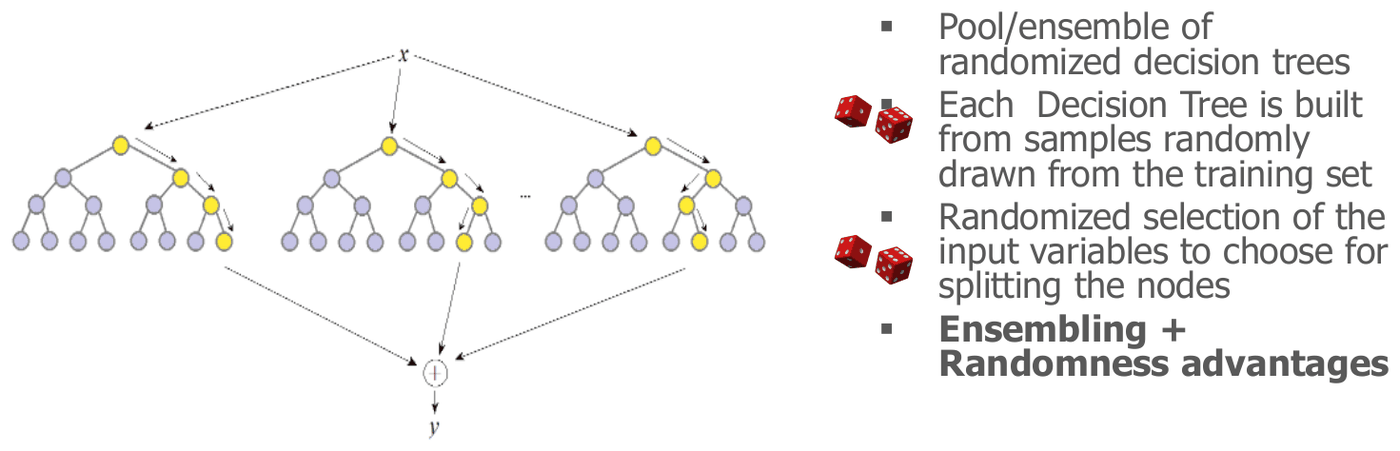
\includegraphics[width=0.71\linewidth,height=0.42\textheight,keepaspectratio]{images/18-rand_random-forest.png}
\caption{Random Forest: an ensemble of randomised decision trees.}
\end{figure}

\section{Random-weight neural networks}\label{reti-neurali-a-pesi-casuali}

\begin{boxquestion}{The question}

Is it possible to exploit MLP (or recurrent) architectures
\textbf{without long training cycles} of the hidden layers?

\end{boxquestion}

There is a long tradition of randomised, random-weight, random
projection networks: for example the \textbf{Random Vector Functional
Link} (RVFL), from the very beginning. Recently they have been
popularised under various names, including \textbf{ELM} (\emph{Extreme
Learning Machine}).

\begin{boxdefinition}{Basic idea}

\begin{itemize}
\tightlist
\item
  A network with one (or more) \textbf{randomly connected hidden
  layers}: the weights are \textbf{fixed after random initialisation}
  and are no longer trained.
\item
  \textbf{Only the output weights} are trained (a linear model: with
  the pseudoinverse or ridge regression).
\end{itemize}

This overcomes the problems of the complex and computationally
expensive training algorithms traditionally used for neural networks.

\end{boxdefinition}

The roots lie in Rosenblatt's pioneering work on the
\textbf{Perceptron}, in which a ``projection'' area randomly connected
to the retina fed an ``association'' area, and only the final responses
were learned. Other pioneering works had stressed the importance of
learning in the output layer compared to the hidden one.

\begin{figure}[htbp]
\centering
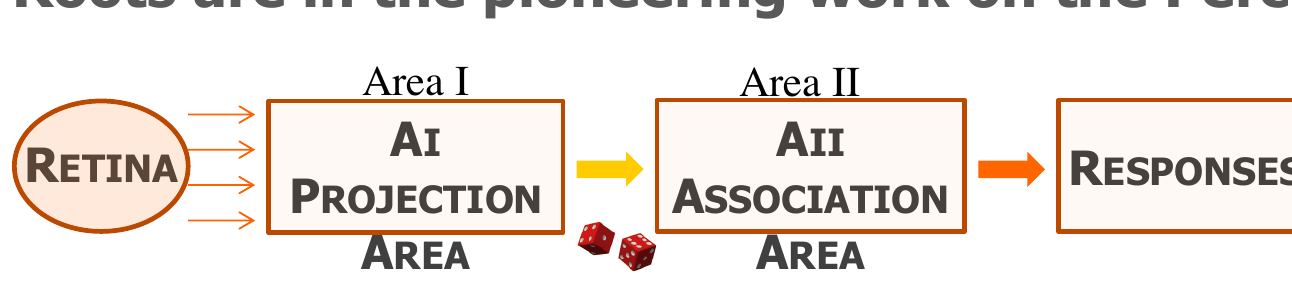
\includegraphics[width=0.69\linewidth,height=0.42\textheight,keepaspectratio]{images/18-rand_perceptron.png}
\caption{The original Perceptron: the connections from the retina to the
projection area were random.}
\end{figure}

Randomised networks are today a growing line of research, particularly
suitable when \textbf{efficiency} is fundamental (training is limited
to the last layer).

\subsection{General structure}\label{struttura-generale}

\begin{figure}[htbp]
\centering
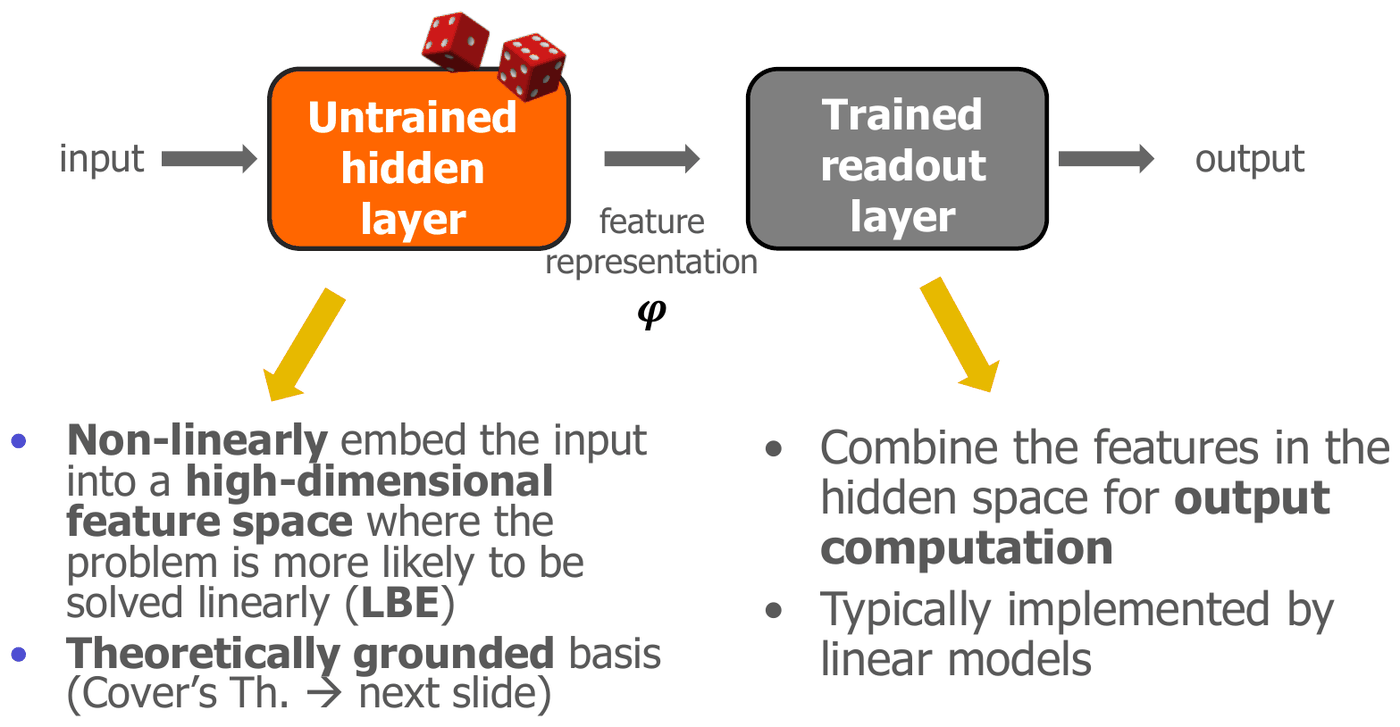
\includegraphics[width=0.80\linewidth,height=0.42\textheight,keepaspectratio]{images/18-rand_struttura.png}
\caption{General structure: an untrained (random) hidden layer and a
trained readout layer.}
\end{figure}

\begin{itemize}
\tightlist
\item
  \textbf{Hidden layer (untrained)}: it \textbf{non-linearly} embeds
  the input in a \textbf{high-dimensional feature space}, where the
  problem is more likely to be linearly solvable (it is an
  \textbf{LBE}!). It has a theoretical basis in Cover's theorem.
\item
  \textbf{Readout (trained)}: it combines the features of the hidden
  space to compute the output; typically it is a \textbf{linear
  model}.
\end{itemize}

\begin{boxtheorem}{Cover's theorem (1965)}

\emph{``A complex pattern-classification problem, cast in a
high-dimensional space non-linearly, is more likely to be linearly
separable than in a low-dimensional space, provided that the space is
not densely populated.''}

For example, with a deterministic mapping: given \(l\) examples, they
are lifted onto the vertices of an \((l-1)\)-dimensional simplex (the
generalised ``triangle''). Now \textbf{every} binary partition of the
samples is linearly separable.

\end{boxtheorem}

It is exactly the same property exploited by \textbf{kernels} in SVMs.

\subsection{Randomised feedforward
networks}\label{reti-feedforward-randomizzate}

\begin{figure}[htbp]
\centering
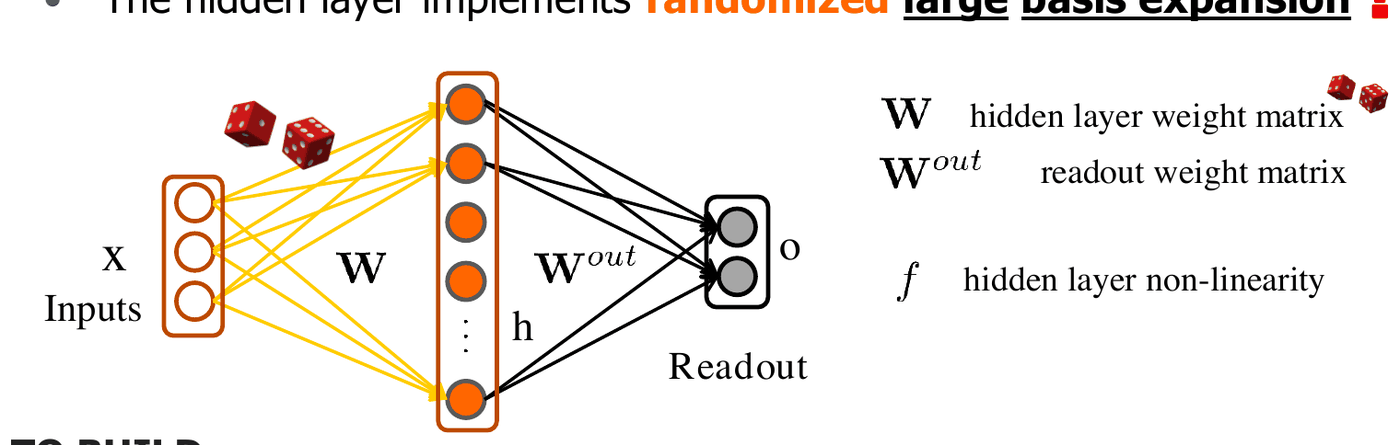
\includegraphics[width=0.80\linewidth,height=0.42\textheight,keepaspectratio]{images/18-rand_rete.png}
\caption{Randomised feedforward network: \(\mathbf{W}\) (random, fixed)
and \(\mathbf{W}^{out}\) (trained).}
\end{figure}

The input-output relationship is implemented by an untrained hidden
layer, which realises a \textbf{large random basis expansion}.

\begin{boxabstract}{Construction, learning and use}

\textbf{Construction}: fill \(\mathbf{W}\) with random values (for
example Gaussian noise), using \textbf{many units}.

\textbf{Learning} of the readout: given \(l\) examples
\((\mathbf{x}_p, \mathbf{d}_p)\), as for linear models the squared
error is minimised with the direct method. With
\(\mathbf{H} = f(\mathbf{W}\mathbf{X})\) (the hidden activations of all
patterns): \[
\mathbf{W}^{out} = \mathbf{H}^+\mathbf{d},
\] often with \textbf{\(L^2\) regularisation} (useful because of the
high number of units): \[
\mathbf{W}^{out} = (\mathbf{H}^T\mathbf{H} + \lambda\mathbf{I})^{-1}\mathbf{H}^T\mathbf{d},
\] or with \(L^1\).

\textbf{Use}: the hidden activations \(\mathbf{h}\) are computed as for
ordinary neurons and then the outputs \[
\mathbf{o}(\mathbf{x}) = \mathbf{W}^{out} f(\mathbf{W}\mathbf{x}),
\] possibly applying a threshold (or a non-linear function) for
classification.

\end{boxabstract}

The main reference models are the \textbf{RVFL} (\emph{Random Vector
Functional-Link}), the \textbf{ELM} (\emph{Extreme Learning Machine})
and \textbf{RBF networks with random centres}.

\begin{boxtip}{Why it works}

Compare with ``ordinary'' neural networks: there the hidden layer is an
\textbf{adaptive} basis expansion \(\phi_j(\mathbf{x}, \mathbf{w})\)
whose weights are learned; here it is a \textbf{random} but very
\textbf{wide} basis expansion. If the bases are numerous enough, by
Cover's theorem the problem becomes (almost) linearly separable in the
hidden space, and a linear output model is enough, trainable in a
single step with least squares. The training cost is that of a
regularised linear regression.

\end{boxtip}

\subsection{Pros and cons}\label{pro-e-contro}

\begin{itemize}
\tightlist
\item
  The large set of hidden units plays an interesting role: the
  projection non-linearly expands the input dimension, making the data
  more separable.
\item
  A high number of units can provide a \textbf{sufficient} basis
  expansion for the task (with theoretical foundations, including
  universal approximation theorems).
\item
  \textbf{Extremely efficient}.
\item
  There are many variants: incremental learning by adding neurons (like
  Cascade Correlation), pruning, etc., often related to past research
  under different names.
\item
  ``Targeted'' models, with fewer adaptive units trained on the
  specific task, nonetheless seem \textbf{more elegant}: there is a
  debate between \textbf{random feature} and \textbf{learned feature}
  approaches, and it is worth knowing both.
\item
  They extend to recurrent networks: \textbf{Echo State Networks}
  (ESN), see
  \href{20\%20-\%20Reti\%20neurali\%20ricorrenti\%20(RNN)}{20 -
  Recurrent neural networks (RNN)}.
\end{itemize}

\subsection{Where they are useful}\label{dove-sono-utili}

\begin{itemize}
\tightlist
\item
  \textbf{Big Data}, thanks to their extreme efficiency.
\item
  Tiny implementations for \textbf{embedded} and distributed systems,
  on resource-constrained devices (sensor networks, IoT, edge
  computing).
\item
  \textbf{Deep learning}, where training algorithms are particularly
  expensive: randomised networks alleviate the computational load
  (randomised deep networks as stacks of RVFL/ELM modules, randomised
  CNNs).
\item
  \textbf{Randomised recurrent networks}: where training is even more
  expensive than for MLPs, and with solid theoretical foundations on
  the bias introduced by the system dynamics (stability,
  learnability).
\end{itemize}

\begin{boxabstract}{Conclusions}

\textbf{Randomness is not an enemy: it is a friend, if it is
controlled.} (This also holds in other fields of computer science, such
as randomised algorithms, and in mathematics.) Note how the same
concepts keep coming back --- Cover's theorem, LBE, regularisation,
feature representation: the course is now ``mature''.

\end{boxabstract}

\begin{boxnote}{FAQ: can ELMs be used in the project?}

Yes, but as an \textbf{additional part} with respect to the standard
implementation of an MLP fully trained with backpropagation and SGD.
They are easy to implement as a sub-part of a feedforward network.

\end{boxnote}

\begin{boxquestion}{Possible exam questions}

\begin{itemize}
\tightlist
\item
  At which levels does randomness appear in ML?
\item
  Describe a randomised feedforward network: construction, readout
  training, use.
\item
  State Cover's theorem and explain its link with randomised networks
  and with kernels.
\item
  Pros and cons of random features compared to learned features.
\end{itemize}

\end{boxquestion}
